\begin{figure}[htbp]
\centering
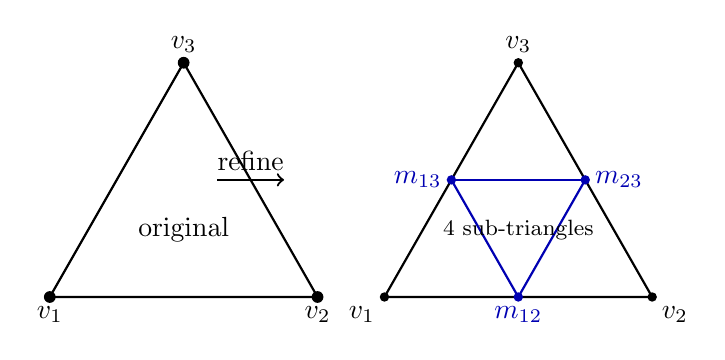
\begin{tikzpicture}[scale=0.85]
  \begin{scope}[xshift=-3cm]
    \draw[thick] (0,0)--(4,0)--(2,3.5)--cycle;
    \fill (0,0) circle (2.5pt) node[below] {$v_1$};
    \fill (4,0) circle (2.5pt) node[below] {$v_2$};
    \fill (2,3.5) circle (2.5pt) node[above] {$v_3$};
    \node at (2,1) {original};
  \end{scope}
  \draw[->,thick] (-0.5,1.75)--(0.5,1.75);
  \node[above] at (0,1.75) {refine};
  \begin{scope}[xshift=2cm]
    \draw[thick] (0,0)--(4,0)--(2,3.5)--cycle;
    \draw[blue!70!black,thick] (2,0)--(3,1.75);
    \draw[blue!70!black,thick] (1,1.75)--(3,1.75);
    \draw[blue!70!black,thick] (1,1.75)--(2,0);
    \fill (0,0) circle (2pt) node[below left] {$v_1$};
    \fill (4,0) circle (2pt) node[below right] {$v_2$};
    \fill (2,3.5) circle (2pt) node[above] {$v_3$};
    \fill[blue!70!black] (2,0) circle (2pt) node[below] {$m_{12}$};
    \fill[blue!70!black] (3,1.75) circle (2pt) node[right] {$m_{23}$};
    \fill[blue!70!black] (1,1.75) circle (2pt) node[left] {$m_{13}$};
    \node at (2,1) {\footnotesize 4 sub-triangles};
  \end{scope}
\end{tikzpicture}
\caption{1-to-4 triangle refinement: each edge is split at its midpoint, producing four congruent sub-triangles.}
\label{fig:mesh_refinement}
\end{figure}
